本章对定理 \ref{thm:direct-HMB} 的一轨道解进行数值求值, 展示三个场的空间分布及传播特征. 所用场值均由无反射留数系统求出, 光场和介质分别按 \eqref{eq:qfinite}、\eqref{eq:RfromM} 重构.

\section{散射数据与三场分布}
取背景和离散参数
\begin{equation}\label{eq:numerical-parameters}
Q=1,\quad a=2,\quad\eta_0=0.6,\quad
\alpha=1,\quad\beta=0.1,\quad b=1.5,
\end{equation}
范数常数按式 \eqref{eq:onec} 确定. 对每个 $(x,z)$, 直接组装式 \eqref{eq:one-AB} 对应的四阶块系统, 用两个右端项求出两组正则列, 再由部分分式表示计算 $M$. 绘图采用双精度线性代数, 各行先作尺度平衡; 介质保留复数计算结果, 并在求值后检查 $\eta$ 的虚部.

图 \ref{fig:one} 在 $x\in\lbrack-6,6\rbrack$、$z\in\lbrack-1.5,1.5\rbrack$ 上使用 $401\times251$ 网格. 光场在非零背景上形成局域振荡结构, 极化与粒子数反转在相同区域发生变化. 参数 \eqref{eq:numerical-parameters} 下 Bloch 长度平方为 $0.45$, 网格最大偏差小于 $7.78\times10^{-16}$, $\eta$ 虚部的最大绝对值小于 $5.21\times10^{-16}$.
\begin{figure}[htbp]
\centering
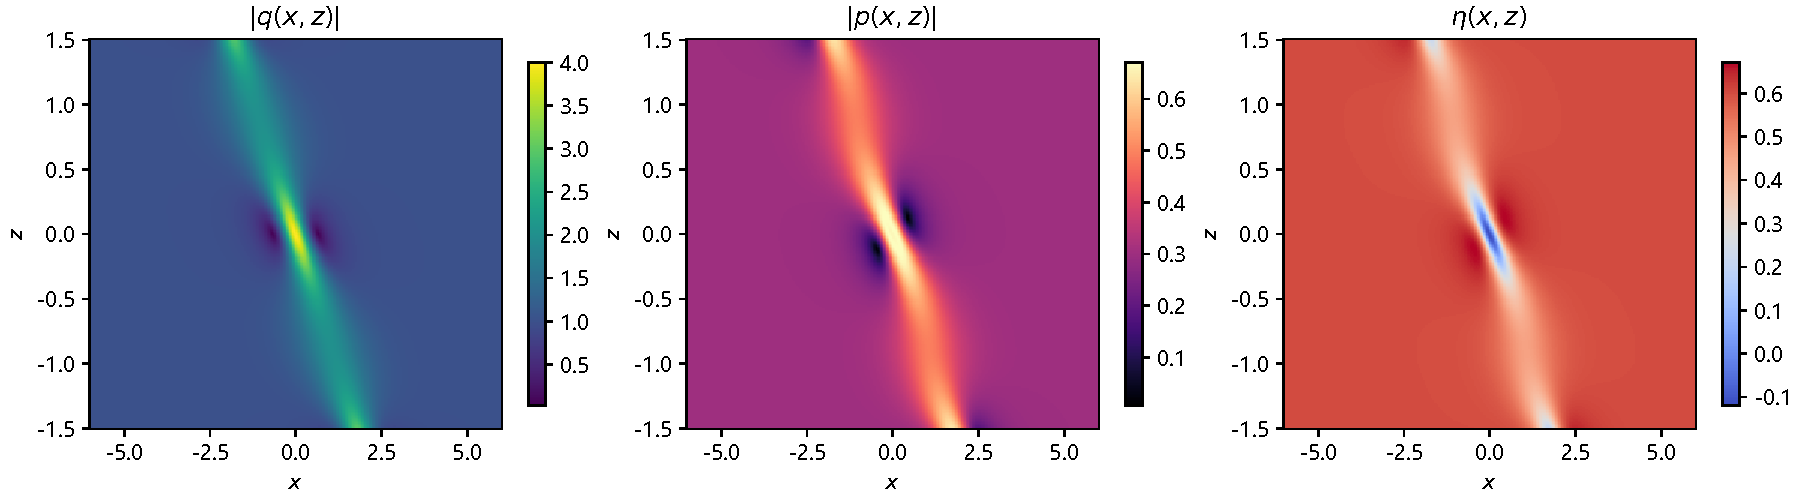
\includegraphics[width=\textwidth]{figures/one-soliton-fields.pdf}
\caption{由一轨道无反射留数系统重构的 $|q|,|p|,\eta$. 参数见 \eqref{eq:numerical-parameters}; 横轴为 $x$, 纵轴为 $z$.}
\label{fig:one}
\end{figure}

\section{传播速度与内部振荡}
由式 \eqref{eq:velocity}、\eqref{eq:frequency}, 上述参数给出
\[
A_b=-1.196,\qquad B_b=-1.572,\qquad
\kappa=\dfrac{\sqrt{5}}{2},\qquad T_z\approx1.78748466439.
\]
图 \ref{fig:dynamics} 左图比较 $z=0,\dfrac{T_z}{4},\dfrac{T_z}{2}$ 时的随动截面. 它们的差异来自式 \eqref{eq:hyperbolic-projector} 中的内部相位, 而局域化尺度由 $\kappa$ 决定. 右图在 $X=0$ 上改变 $\alpha$, 其余参数固定. 对应的解析频率和周期列于表 \ref{tab:periods}. 当 $\alpha=-0.048=-\dfrac{\eta_0}{a(a^2+b^2)}$ 时 $B_b=0$, 去相位三场为行波; 当 $B_b\ne0$ 时, 中心光场模随传播变量周期变化.
\begin{table}[htbp]
\centering
\caption{改变 $\alpha$ 时的随动内部频率与周期, 其余参数同 \eqref{eq:numerical-parameters}}
\label{tab:periods}
\begin{tabular}{cccc}
\toprule
$\alpha$ & $A_b$ & $B_b$ & $T_z$\\
\midrule
$-0.048$ & $-1.196$ & $0$ & 行波\\
$0.5$ & $-1.196$ & $-0.822$ & $3.41840132897$\\
$1$ & $-1.196$ & $-1.572$ & $1.78748466439$\\
\bottomrule
\end{tabular}
\end{table}
\begin{figure}[htbp]
\centering
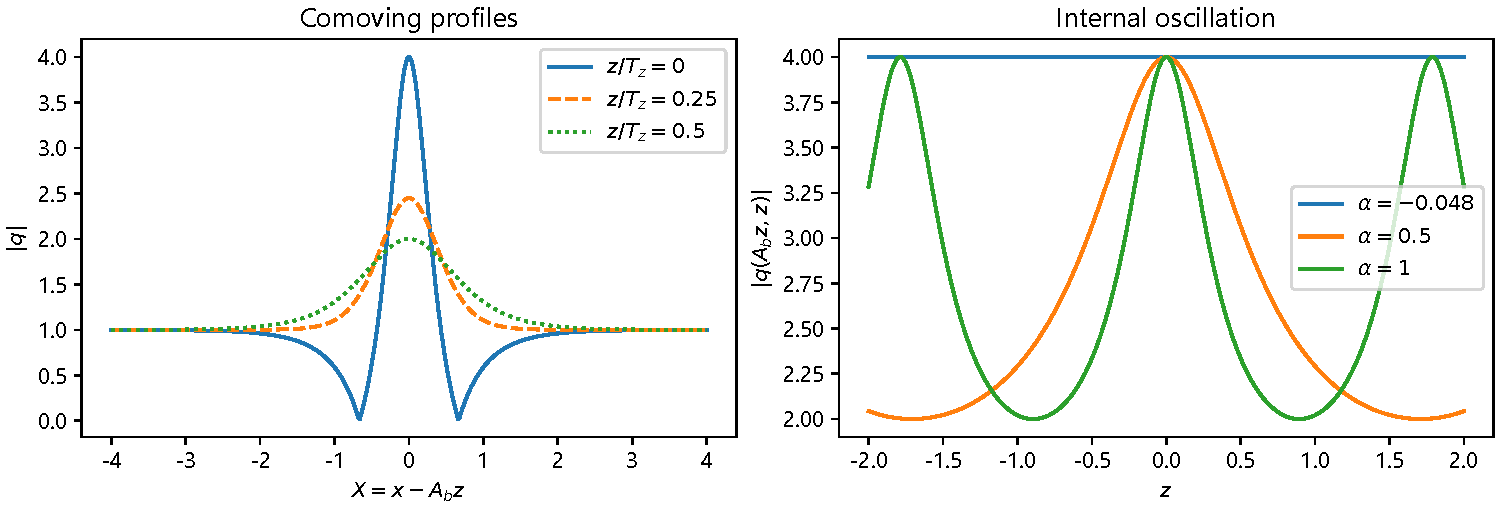
\includegraphics[width=\textwidth]{figures/one-soliton-dynamics.pdf}
\caption{一轨道光场的随动截面与内部振荡. 左图为基础参数下的三个截面, 右图为不同 $\alpha$ 下 $|q(A_bz,z)|$ 的变化.}
\label{fig:dynamics}
\end{figure}

参数 $\beta$ 出现在 $A_b$ 中, 不出现在 $B_b$ 中. 图 \ref{fig:velocity} 取 $\beta=0,0.15$, 对应速度分别为 $-0.096,-1.746$, 而两者均有 $B_b=-1.572$ 和相同的随动周期. 图中的虚线 $x=A_bz$ 给出随动坐标的中心轨迹. 这与命题 \ref{prop:wave-properties} 对传播平移和内部相位的分离一致.
\begin{figure}[htbp]
\centering
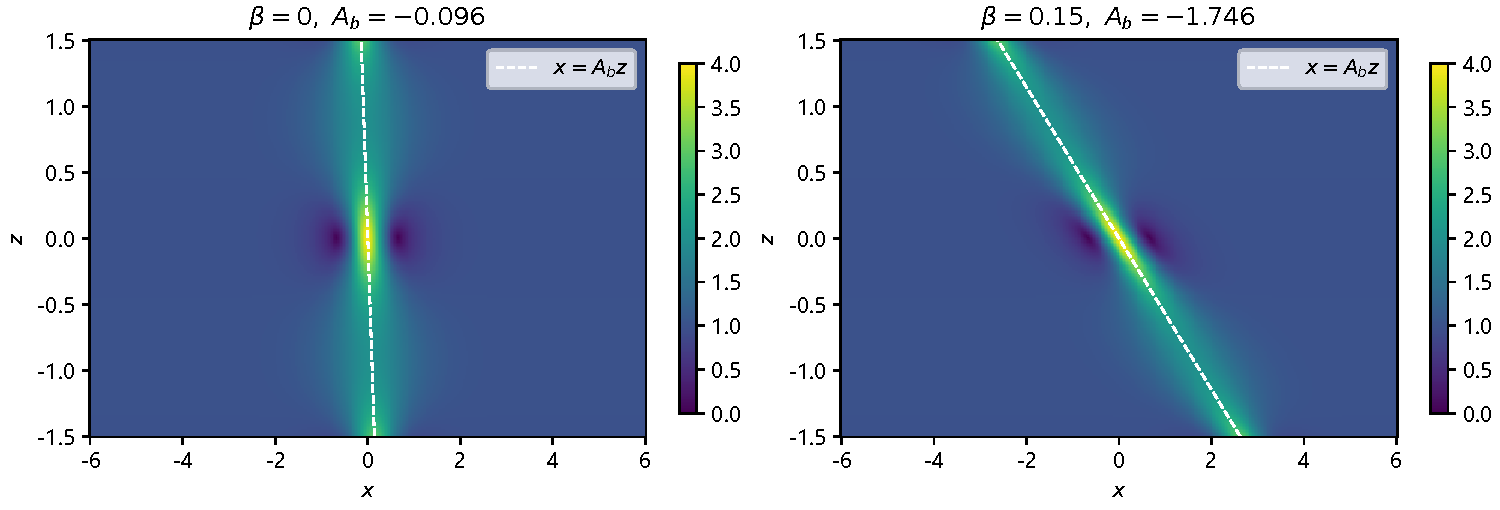
\includegraphics[width=\textwidth]{figures/one-soliton-velocity.pdf}
\caption{$\beta$ 对光场传播速度的影响. 两图分别取 $\beta=0,0.15$, 其余参数同 \eqref{eq:numerical-parameters}; 白色虚线为 $x=A_bz$.}
\label{fig:velocity}
\end{figure}

\section{精确参数例的代数检验}
作为一轨道公式的精确代数例, 取
\begin{equation}\label{eq:exactparams}
Q=1,\quad b=\dfrac{5}{4},\quad\kappa=\dfrac{3}{4},\quad
a=2,\quad\eta_0=\dfrac{3}{5},\quad\alpha=1,\quad\beta=\dfrac{1}{10}.
\end{equation}
此时 $h_0=\dfrac{1}{2}$, $F(\ii b)=-\dfrac{3321}{3560}-\dfrac{469\ii}{356}$. 令
$T=e^{2\operatorname{Re}s}>0$、$C=e^{2\ii\operatorname{Im}s}$, 则 $t=TC$、$\conj t=\dfrac{T}{C}$, 且
\[
\Delta_-=\dfrac{5}{4}(T^2+1)-T(C+C^{-1}).
\]
式 \eqref{eq:direct-vu1}--\eqref{eq:direct-vu2} 因而都是 $T,C$ 的有理式, 原方程可按
\[
\partial_x=2\kappa T\partial_T,\qquad
\partial_z=-2\kappa\operatorname{Re}F\,T\partial_T
-2\ii\kappa\operatorname{Im}F\,C\partial_C
\]
作精确检验. 代入式 \eqref{eq:finalfields} 后, 三条 PDE 的有理残差均为零, 且 $|p|^2+\eta^2=\dfrac{9}{20}$. 在 $T>0,|C|=1$ 上分母严格正, 清分母不引入额外解.


\section{高精度重构与方程残差}
对参数 \eqref{eq:numerical-parameters}, 采用 70 位十进制精度直接求解留数系统. 在五个时空点
\[
(-1.2,-0.35),\quad(0,0),\quad(0.37,0.21),\quad
(1.4,-0.1),\quad(2.3,0.6)
\]
对重构表达式作高精度微分, 得到表 \ref{tab:direct-residuals} 的最大绝对残差. 微分作用于线性系统的解及重构式, 三条 PDE 的右端用于计算残差. 矩阵检验另取三个普通谱点 $w=2.1+0.7\ii$、$0.3-0.2\ii$ 和 $1.2$.
\begin{table}[htbp]
\centering
\caption{五点采样下的独立重构检验, 数值均向上舍入}
\label{tab:direct-residuals}
\begin{tabular}{lc}
\toprule 检验对象 & 最大绝对误差\\\midrule
光场方程 & $1.87\times10^{-69}$\\
极化方程 & $8.26\times10^{-71}$\\
粒子数反转方程 & $1.50\times10^{-70}$\\
空间 Lax 方程 & $4.82\times10^{-70}$\\
传播 Lax 方程 & $1.95\times10^{-69}$\\
两个共振原像的介质重构 & $9.71\times10^{-72}$\\
Bloch 长度平方 & $9.07\times10^{-72}$\\
\bottomrule
\end{tabular}
\end{table}

同一组采样点上, 绘图实现与高精度实现的三个场最大差分别小于 $6.01\times10^{-16}$、$1.99\times10^{-16}$、$2.23\times10^{-16}$. 固定 $z=0.21$, 在 $x=\pm30$ 处检查式 \eqref{eq:targetboundary} 的三个端态, 最大误差小于 $5.02\times10^{-29}$. 留数、两种谱约化、行列式、归一化及分支点固定核也由同一矩阵逐项检验.
